\documentclass[pdf,mathserifaspectratio=169]{beamer} % , a4, handout
\usepackage[orientation=landscape,size=custom,width=16,height=9,scale=0.5,debug]{beamerposter}
\usepackage{etex}
\usetheme{ltg}

\usepackage{textcomp}
\usepackage{ifpdf}
\usepackage{pxfonts}
\usepackage[american]{babel} 
\usepackage[utf8]{inputenc}
\usepackage{lmodern}
\usepackage[T1]{fontenc}
\usepackage{relsize}
\usepackage{amsmath}
\usepackage{multirow}
\usepackage{booktabs}
\usepackage{colortbl}
\usepackage{xcolor}
\usepackage{thumbpdf}
\usepackage{graphicx}
\usepackage{fancybox}
\usepackage{hyperref}
\usepackage{textcomp}
\usepackage{pdfpages}
\usepackage{ulem}
\usepackage{tikz}
\usetikzlibrary{arrows,shapes,backgrounds}
\usepackage{pgfplots,pgfplotstable}
\usepackage{natbib}
\usepackage{apalike}
\bibliographystyle{apalike}
\newcommand{\ntuple}[2]{\ensuremath{\left({#1}_1, {#1}_2, \ldots, {#1}_{#2}\right)}}
\newcommand{\vect}[1]{\ensuremath{\boldsymbol{#1}}}
\newcommand{\mat}[1]{\ensuremath{\boldsymbol{#1}}}
\newcommand{\func}[1]{\ensuremath{\operatorname{{#1}}}}

\newcommand{\cf}{cf.}
\newcommand{\eg}{e.g.}
\newcommand{\ie}{i.e.}
\newcommand{\etc}{etc.}
\newcommand{\vs}{vs.}
\newcommand{\viz}{viz.}
\newcommand{\etal}{et al.}

\def\argmax{\mathop{\rm arg\,max}}
\def\argmin{\mathop{\rm arg\,min}}
\def\fscore{F$_1$}


\usepackage{latexsym}
\usepackage{graphics}
\usepackage{color}
\usepackage{fancyvrb}
\usepackage{adjustbox}

\usepackage{pifont}\newcommand{\cmark}{\ding{51}}\newcommand{\xmark}{\ding{55}}

\newfont{\titlehvr}{phvr at 48pt}

\definecolor{oe}{rgb}{0,0,1}
\definecolor{DarkBlue}{rgb}{0.1,0.1,0.5}
\definecolor{LightGreen}{rgb}{0.1,0.5,0.1}
\definecolor{DarkGreen}{rgb}{0,0.2,0}
\definecolor{Red}{rgb}{0.9,0.0,0.1}
\definecolor{Dandelion}{cmyk}{0,0.25,0.84,0}
\definecolor{lgray}{gray}{0.85}
\definecolor{mgray}{gray}{0.4}
\definecolor{light}{gray}{.2}

\fboxsep 0pt
\pgfdeclareimage[height=8mm]{logo}{graphics/logo}
\usepackage[many]{tcolorbox}
\usepackage[absolute,overlay]{textpos}
\setlength{\TPHorizModule}{1mm}
\setlength{\TPVertModule}{1mm}
\newcommand{\includelogo}{%
  \begin{textblock}{10}(153,0.25)\pgfuseimage{logo}\end{textblock}}

\begin{document}

%\iffalse
\title[]{Forskning og utvikling for store, åpne språkmodeller i Norge}
\author[]{Yngvil Beyer, Jon Atle Gulla, Lilja Øvrelid, Stephan Oepen\vskip -4ex}
\date[]{\color{DarkBlue}8.\ juni 2026 -- Språkmodeller og digital selvråderett}
\institute[]{}

\begin{frame}[fragile,plain]
  \vskip -1ex
  \centerline{
\includegraphics[height=28mm]{graphics/logo+name}}
  \vskip -2ex
  \titlepage
\end{frame}

\begin{frame}[fragile]\includelogo
  \frametitle{5.\ februar:\ Et fornyet og styrket samarbeid}
  \vskip -1ex
  \begin{columns}
    \begin{column}{.7\textwidth}
      \begin{center}
        \fbox{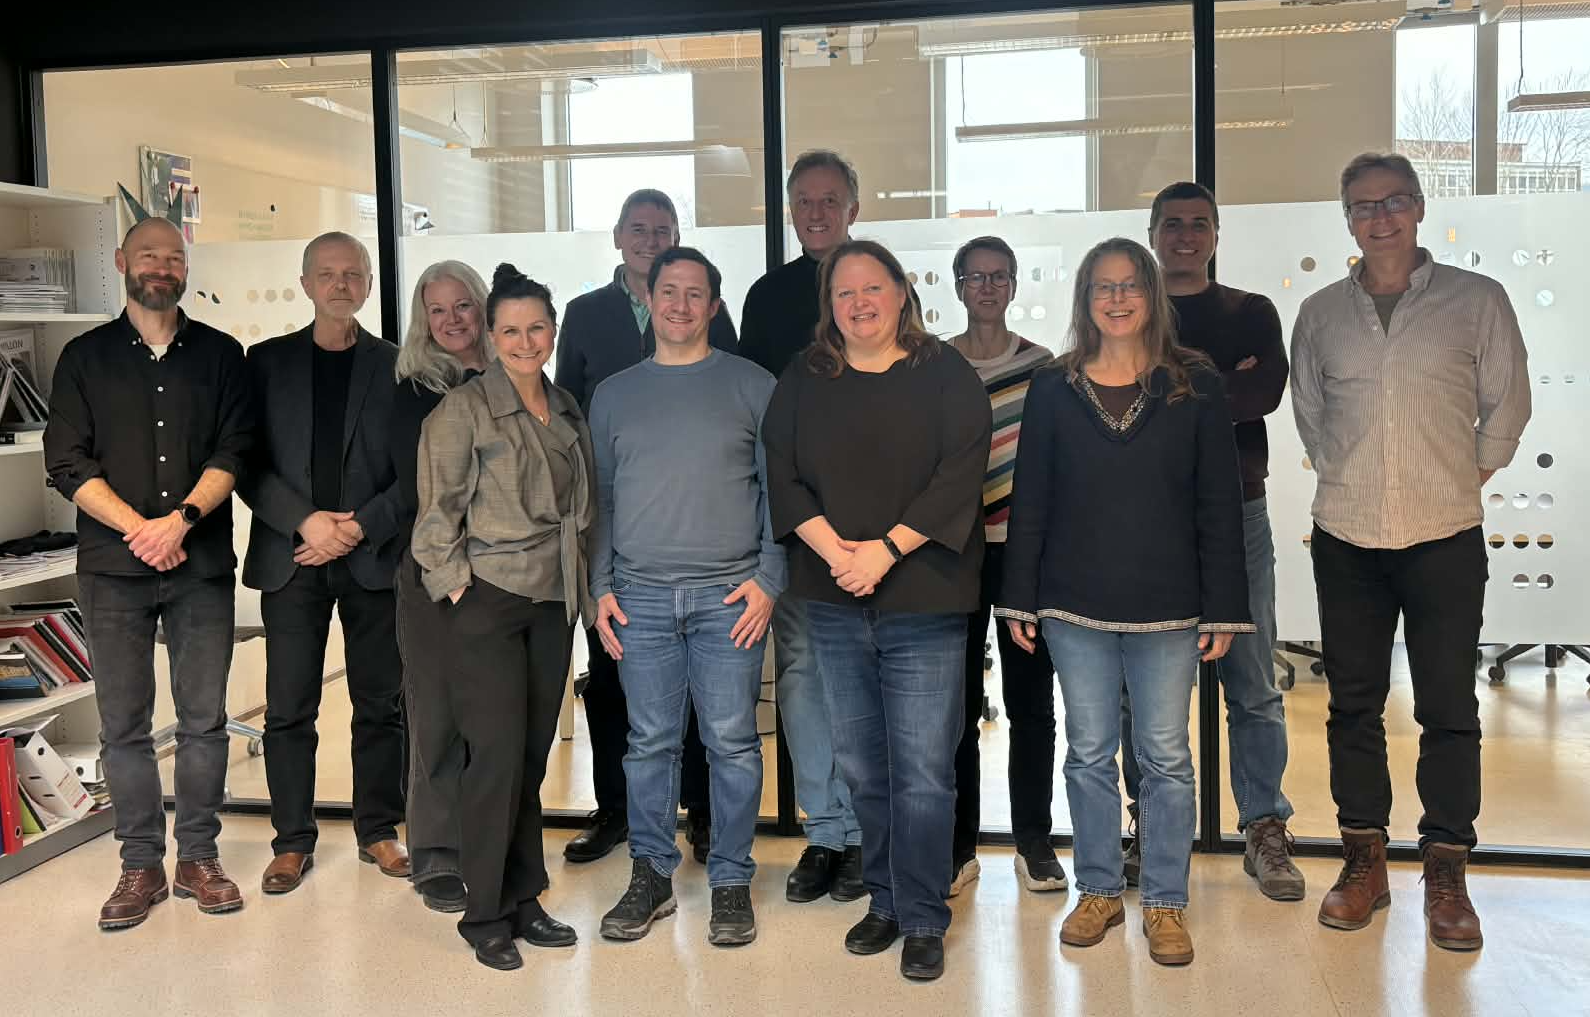
\includegraphics[width=.95\textwidth]{graphics/260205}}\\[1.5ex]
      \end{center}
    \end{column}
    \pause
    \begin{column}{.3\textwidth}
      \begin{center}
        
\includegraphics[width=.95\textwidth]{graphics/nb}\\[1.5ex]
        
\includegraphics[width=.95\textwidth]{graphics/ntnu}\\[1.5ex]
        
\includegraphics[width=.95\textwidth]{graphics/uio}\\[2.5ex]
        \pause
        
\includegraphics[width=.95\textwidth]{graphics/sigma2}\\[1.5ex]
        
\includegraphics[width=.95\textwidth]{graphics/lcn}\\
      \end{center}
    \end{column}
  \end{columns}
\end{frame}

\begin{frame}[fragile]\includelogo
  \frametitle{8.\ juni:\ Nasjonal statusmelding og «Klyngas anbefalinger»}
  \vskip -1ex
  \begin{columns}
    \begin{column}{.7\textwidth}
      \begin{center}
        \fbox{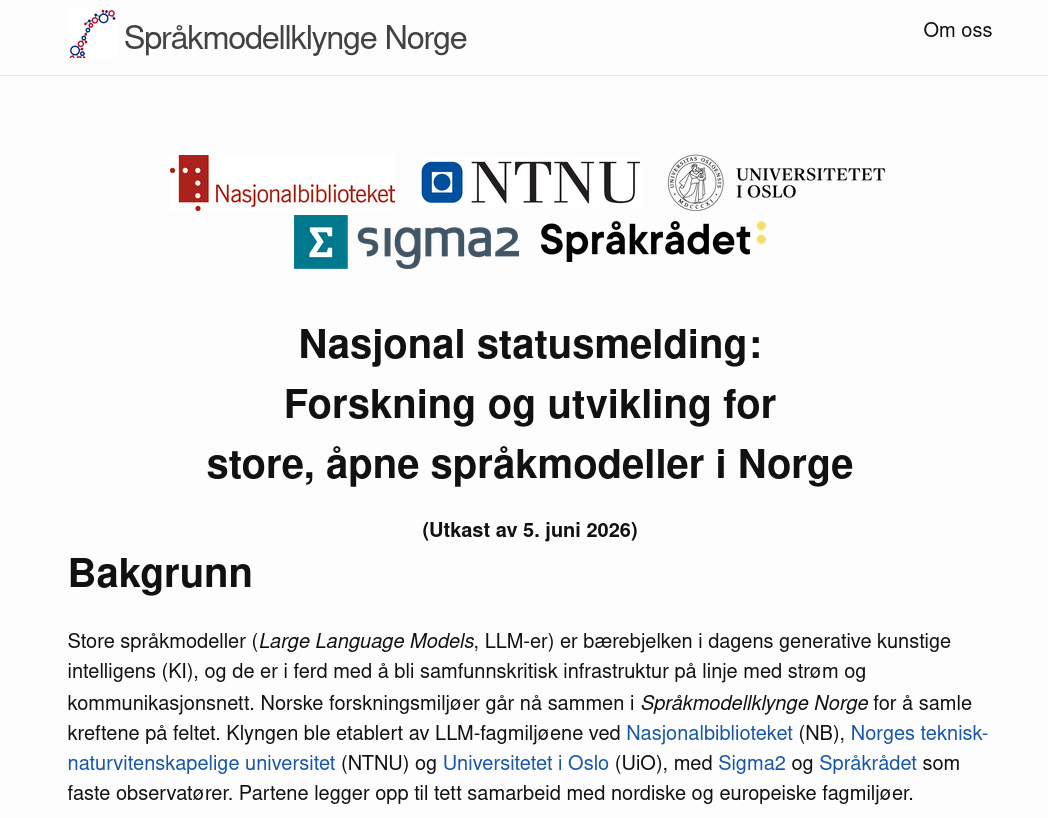
\includegraphics[width=.9\textwidth]{graphics/statusmelding}}\\[1.5ex]
      \end{center}
    \end{column}
    \begin{column}{.3\textwidth}
      \begin{center}
        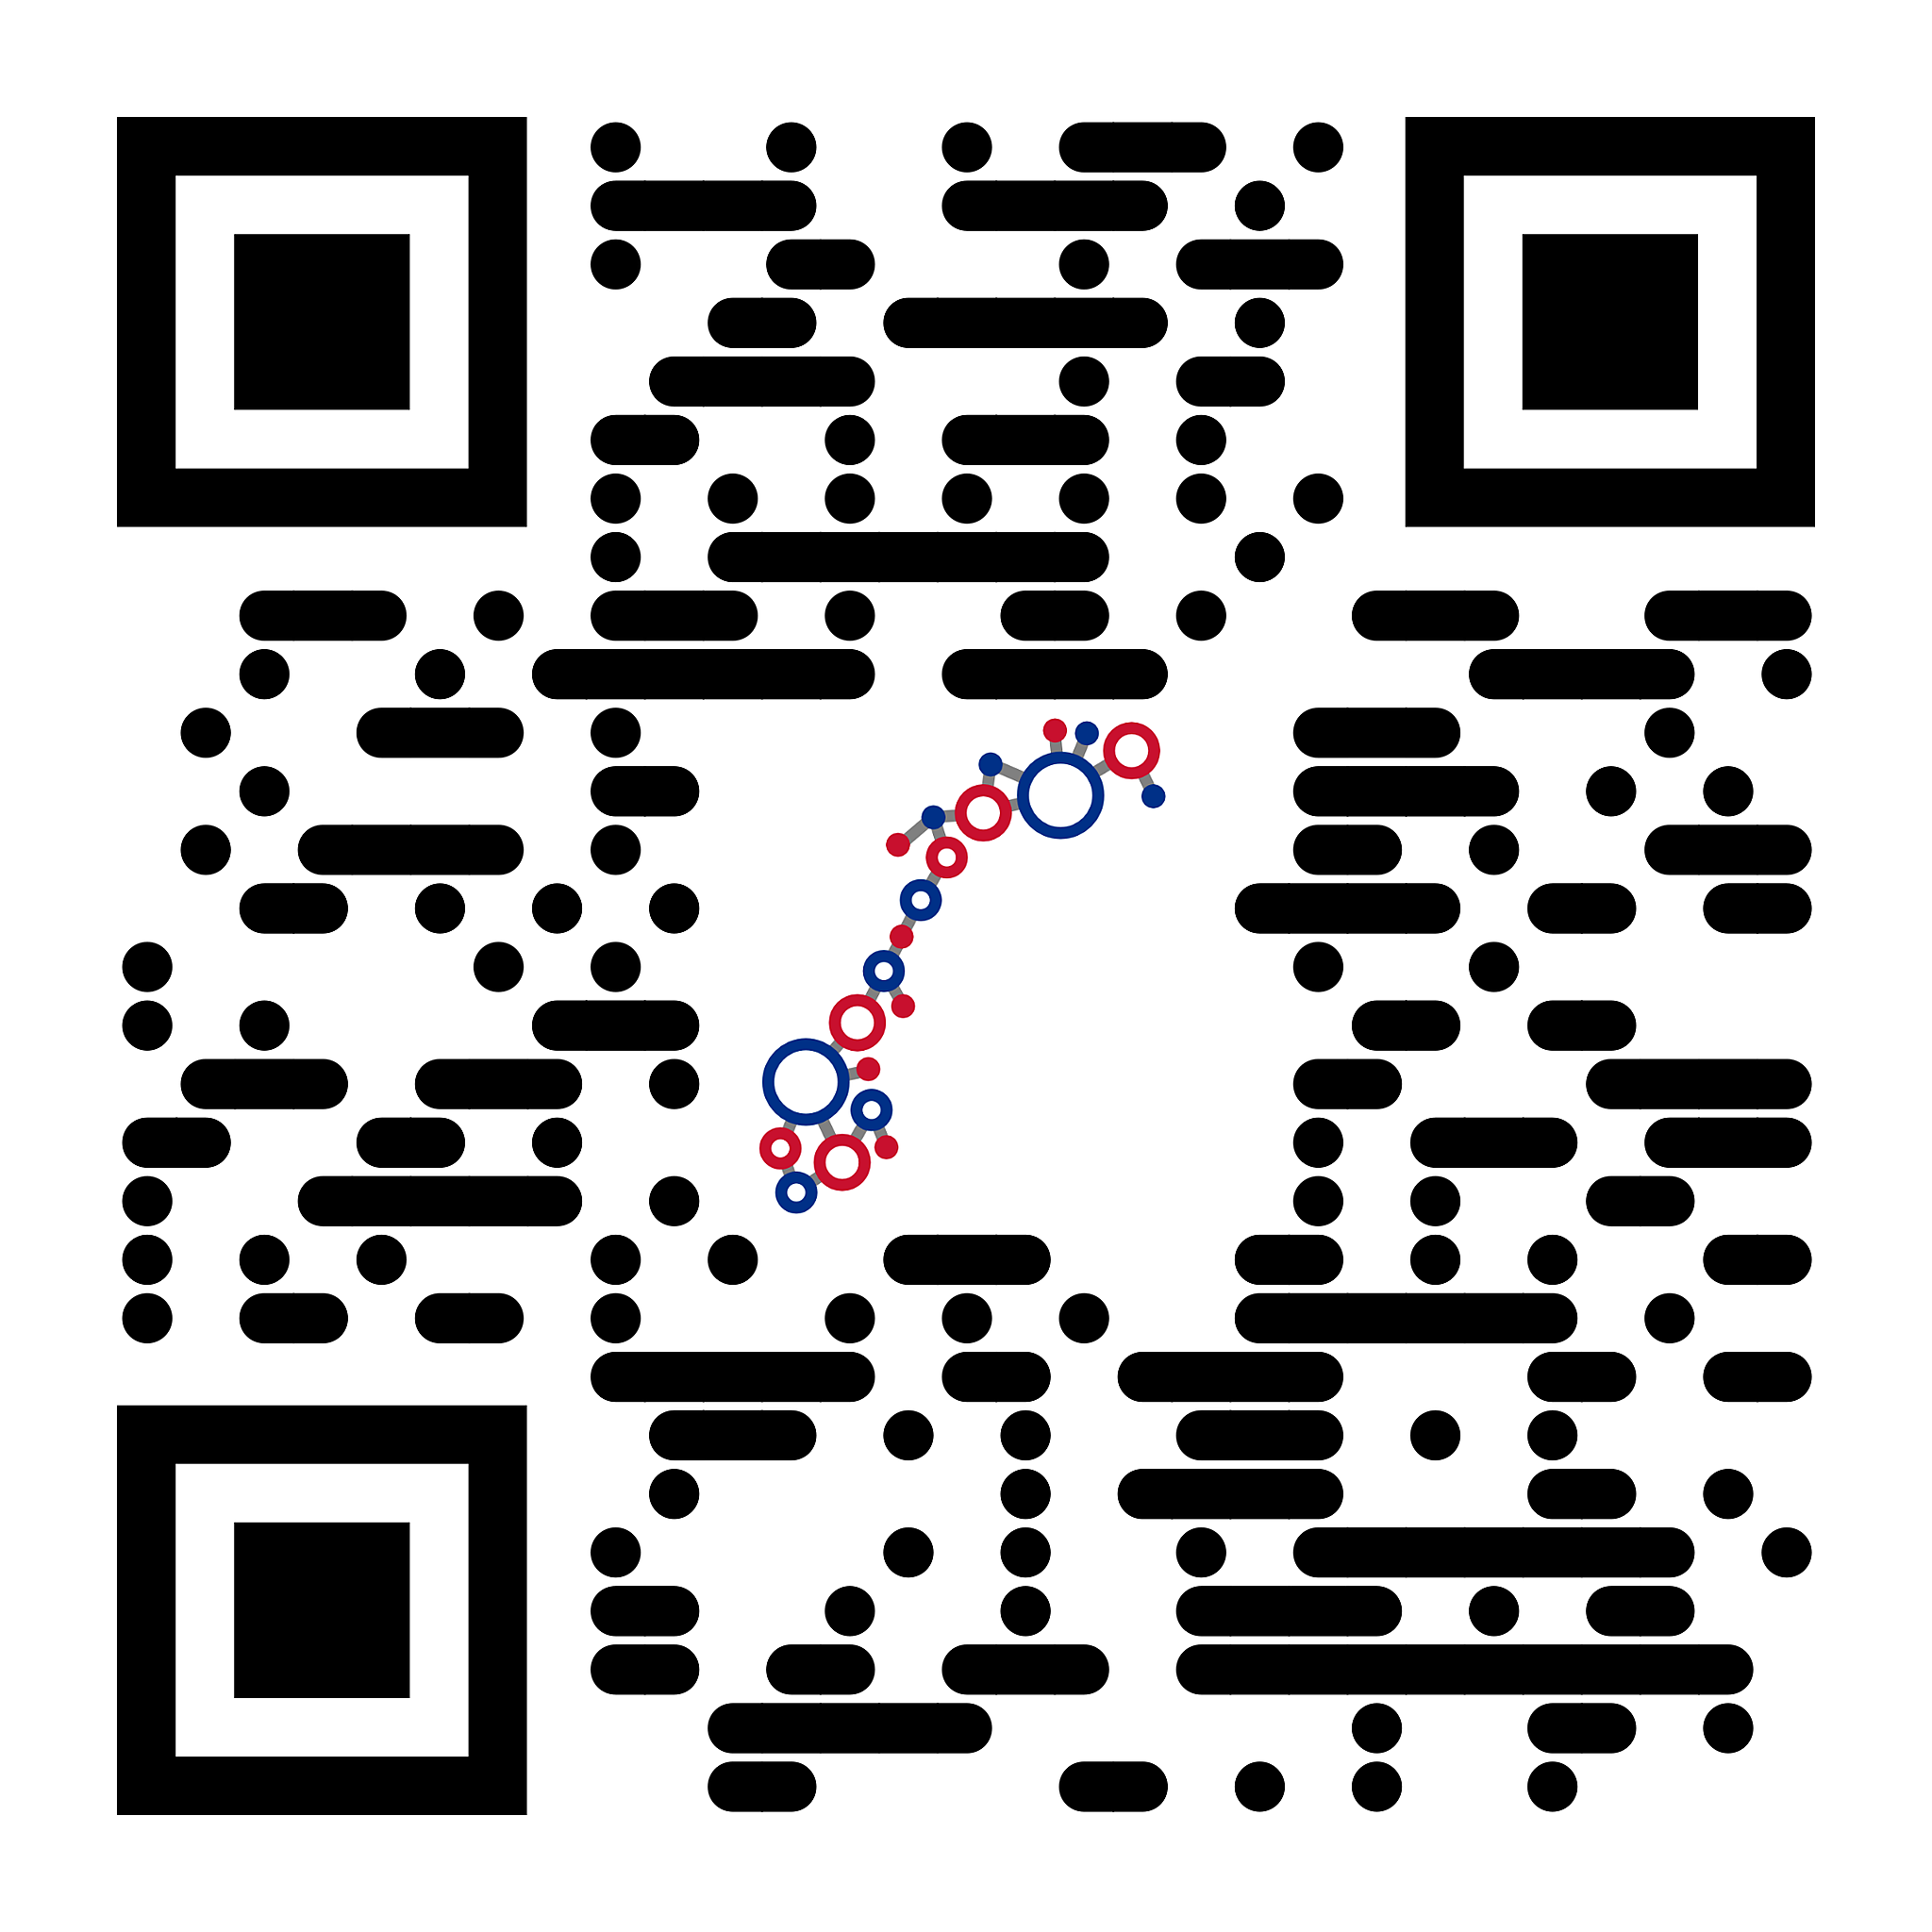
\includegraphics[width=\textwidth]{graphics/qr}\\[1.5ex]
      \end{center}
    \end{column}
  \end{columns}
\end{frame}


\end{document}

\begin{frame}[fragile]\includelogo % oe
  \frametitle{The Consortium:\ 21 Partners, 9 European Countries}
  \begin{center}
    \vspace*{-2.5ex}
    \fboxsep 0pt
    \fbox{\includegraphics[width=\textwidth, page=1, trim={0.6cm 1cm 1.5cm 2cm}, clip]{consortium}}\\[1ex]
  \end{center}
\end{frame}

\begin{frame}[fragile]\includelogo % oe
  \frametitle{The Consortium:\ 21 Partners, 9 European Countries}
  \begin{center}
    \vspace*{-2.5ex}
    \fboxsep 0pt
    \fbox{\includegraphics[width=\textwidth, page=2, trim={0.6cm 1cm 1.5cm 2cm}, clip]{consortium}}\\[1ex]
  \end{center}
\end{frame}

\begin{frame}[fragile]\includelogo % oe
  \frametitle{The Consortium:\ 21 Partners, 9 European Countries}
  \begin{center}
    \vspace*{-2.5ex}
    \fboxsep 0pt
    \fbox{\includegraphics[width=\textwidth, page=3, trim={0.6cm 1cm 1.5cm 2cm}, clip]{consortium}}\\[1ex]
  \end{center}
\end{frame}

%
% three years, about 3800 person months, equivalent to 100 full-time people
% 38 m€ budget, of which 21 m€ EU contribution
% by far largest part is salary costs; compute expected from EuroHPC
%
\begin{frame}[fragile]\includelogo % oe
  \frametitle{The Consortium:\ 21 Partners, 9 European Countries}
  \begin{center}
    \vspace*{-2.5ex}
    \fboxsep 0pt
    \fbox{\includegraphics[width=\textwidth, page=4, trim={0.6cm 1cm 1.5cm 2cm}, clip]{consortium}}\\[1ex]
  \end{center}
\end{frame}

\begin{frame}[fragile]\includelogo % oe
  \frametitle{A Few Faces:\ Work Package Co-Leads}
  \begin{center}
    \vspace*{-.5ex}
    \fboxsep 0pt
    \fbox{\includegraphics[width=.96\textwidth, page=3, trim={0.6cm 0cm 0.2cm 1.1cm}, clip]{drive}}\\[1ex]
  \end{center}
\end{frame}

\begin{frame}[fragile]\includelogo % oe
  \frametitle{Project Lifecycle:\ Preparation -- Production -- Flagship}
  \begin{center}
    \vspace*{1ex}
    \fboxsep 0pt
    \fbox{\includegraphics[width=.97\textwidth, page=2, trim={0.5cm 1.5cm 0.5cm 2.5cm}, clip]{gema}}\\[2.5ex]
    \scshape
    \textcolor{DarkBlue}{collaboration} --
    \textcolor{DarkGreen}{data mixtures} --
    \textcolor{DarkBlue}{infrastructure} --
    \textcolor{DarkGreen}{evaluation}
  \end{center}
\end{frame}

\begin{frame}[fragile]\includelogo % oe
  \frametitle{Two Overlapping Development Cycles in 2026}
  \pause
  \begin{block}{``BABY'':\ First Mid-Size Production Model -- ``Q2'' 2026;}
    \begin{center}\color{DarkGreen}
      Dense, Llama-like, 8B parameters, 10T tokens, 256k tokenizer, Megatron-LM;\\[0.5ex]
      Nemotron-CC, DCLM, FinePDFs(-edu), \alert{HPLT 3.0}, \alert{MultiSynt}, code, math.
    \end{center}
  \end{block}
  \pause
  \begin{block}{``FLAG''\hskip -0.75ex$_\text{dense}$:\ First Dense Flagship Model -- Q4 2026}
    \begin{center}\color{DarkBlue}
      Qwen3-like, 30B parameters, 15T tokens, 256k tokenizer, Megatron-LM;\\[0.5ex]
      similar; \alert{HPLT 4.0}; own \alert{quality filtering}; more \alert{synthetics}, parallel, code, math.
    \end{center}
  \end{block}
  \pause
  \begin{block}{``FLAG''\hskip -0.75ex$_\text{moe}$:\ First Non-Dense Flagship Model -- Q1 2027}
    \begin{center}\color{DarkGreen}
      ``Comparable in scale'', 15T tokens, 256k tokenizer, Megatron-LM;\\[0.5ex]
      same training data mixture as FLAG$_\text{dense}$.
    \end{center}
  \end{block}
  \pause
  \begin{center}
    \scshape
    \textcolor{red}{intensive continual exploratory work on e.g.\\[0.1ex]
      quality signals, data mixtures, scaling laws, evaluation}
  \end{center}
\end{frame}

\begin{frame}[fragile]\includelogo % oe
  \frametitle{At the Core:\ Model Development (WP4)}
  \begin{center}
    \vspace*{-.5ex}
    \fboxsep 0pt
    \fbox{\includegraphics[width=.98\textwidth, page=1, trim={2.3cm 0.2cm 0.4cm 2.5cm}, clip]{drive}}\\[1ex]
  \end{center}
\end{frame}

\begin{frame}[fragile]\includelogo % oe
  \frametitle{The Quest for Compute}
  \begin{center}
    \vspace*{-.5ex}
    \fboxsep 0pt
    \fbox{\includegraphics[width=.99\textwidth, page=1, trim={0cm 0cm 0cm 1.3cm}, clip]{gema}}\\[1ex]
  \end{center}
\end{frame}

\begin{frame}[fragile]\includelogo % oe
  \frametitle{Compute Calculator for ``FLAG''\hskip -0.75ex$_\text{dense}$}
  \begin{center}
    \vspace*{0ex}
    \fboxsep 0pt
    \fbox{\includegraphics[width=.99\textwidth]{graphics/compute}}\\[1.5ex]
    \pause
    \smaller\scshape
    \textcolor{red}{currently (expecting to be) allocated some {\smaller 6.5}m hours on jupiter for {\smaller 2026};\\[0.1ex]
      with optimistic estimates, not quite enough for
      ``flag''\hskip -0.75ex$_\text{dense}$ \& ``flag''\hskip -0.75ex$_\text{moe}$}
  \end{center}
\end{frame}

\begin{frame}[fragile]\includelogo % oe
  \frametitle{For Example:\ Multilingual ``Quality'' Annotation}
  \begin{center}
    \vspace*{-.5ex}
    \fboxsep 0pt
    \fbox{\includegraphics[width=.85\textwidth, trim={0cm 0cm 0cm .6cm}, clip]{graphics/propella}}\\[2.5ex]
  \end{center}
\end{frame}

\begin{frame}[fragile]\includelogo % oe
  \frametitle{For Example:\ Enhancing Multilingual Training Data}
  \begin{center}
    \vspace*{-.5ex}
    \fboxsep 0pt
    \fbox{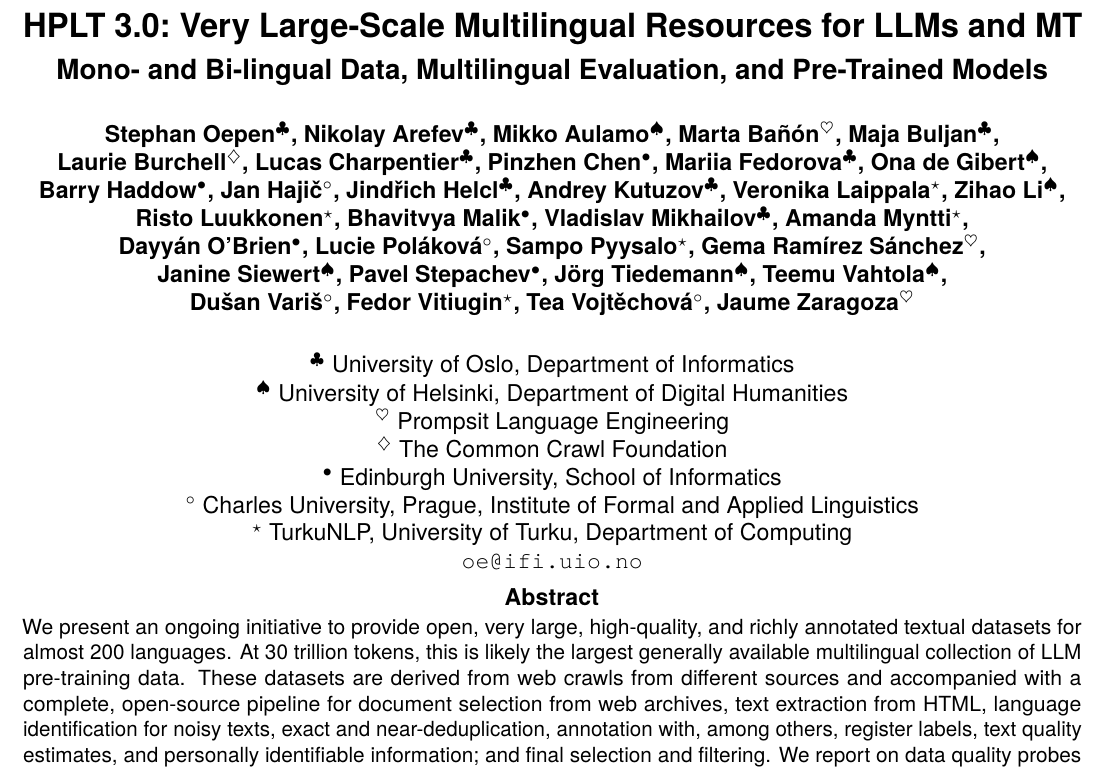
\includegraphics[width=.82\textwidth]{graphics/hplt3}}\\[2.5ex]
  \end{center}
\end{frame}

\begin{frame}[fragile]\includelogo
  \frametitle{Dataset Comparison: Seven Languages (2B--100BT)}
  \begin{center}
    \vspace*{-0.5ex}
    \includegraphics[width=0.7\textwidth]{graphics/hplt-e.png}\\[-0.5ex]
    \textcolor{red}{\url{https://github.com/hplt-project/hplt-e}}
  \end{center}
\end{frame}
%\fi

\begin{frame}[fragile]\includelogo
  \frametitle{Systematic Comparison of Different Quality Signals}
  \begin{columns}
    \begin{column}{0.58\textwidth}
      \includegraphics[width=0.99\textwidth]{graphics/signals}
    \end{column}
    \begin{column}{0.42\textwidth}
      \begin{itemize}\itemsep 8pt
      \item HPLT 4.0 annotated with \alert{five distinct} ``educational'' models;
      \item WDS:\ unified surface heuristics;
      \item JQL:\ six different configurations;
      \item propella:\ eight ordinal properties;
      \pause
      \item overall:\ many \alert{strong correlations};
      \item FinePDFS-edu\raisebox{0.2ex}{\smaller$\,\sim\,$}JQL\raisebox{0.2ex}{\smaller$\,\sim\,$}BSC-edu;
      \item \raisebox{0.2ex}{\smaller$\,\sim\,$}propella:\ educational\_value;
      \item bit of an outlier:\ FineWeb2-HQ.
      \end{itemize}
    \end{column}
  \end{columns}
\end{frame}

\begin{frame}[fragile]\includelogo % oe
  \frametitle{The LLM Dilemma:\ Data Paucity \& Legal Uncertainty}
  \begin{columns}
    \begin{column}{0.33\textwidth}
      \begin{center}
        \vspace*{-2ex}
        \includegraphics[width=0.95\textwidth]{graphics/nno}\\[1ex]
      \end{center}
    \end{column}
    \begin{column}{0.67\textwidth}
      \color{DarkBlue}
      \begin{itemize}\itemsep 4pt
      \item Majority of \alert{web content} is published under \alert{copyright};
      \item like CC \& IA:\ redistribute \alert{without claim of ownership};
      \item best effort to respect \alert{common practices for `opt-out'};
      \item take-down mechanism (removal) by legitimate request;
      \item all metadata and \alert{collections `per se'} licensed as CC0.
      \end{itemize}
      \vspace*{1ex}
      \centerline{\alert{\url{https://hplt-project.org/datasets/v4.0}}}
      \vspace*{1ex}
      \pause
      \begin{center}
        \includegraphics[height=1cm]{graphics/hplt}\hspace*{3.5em}
        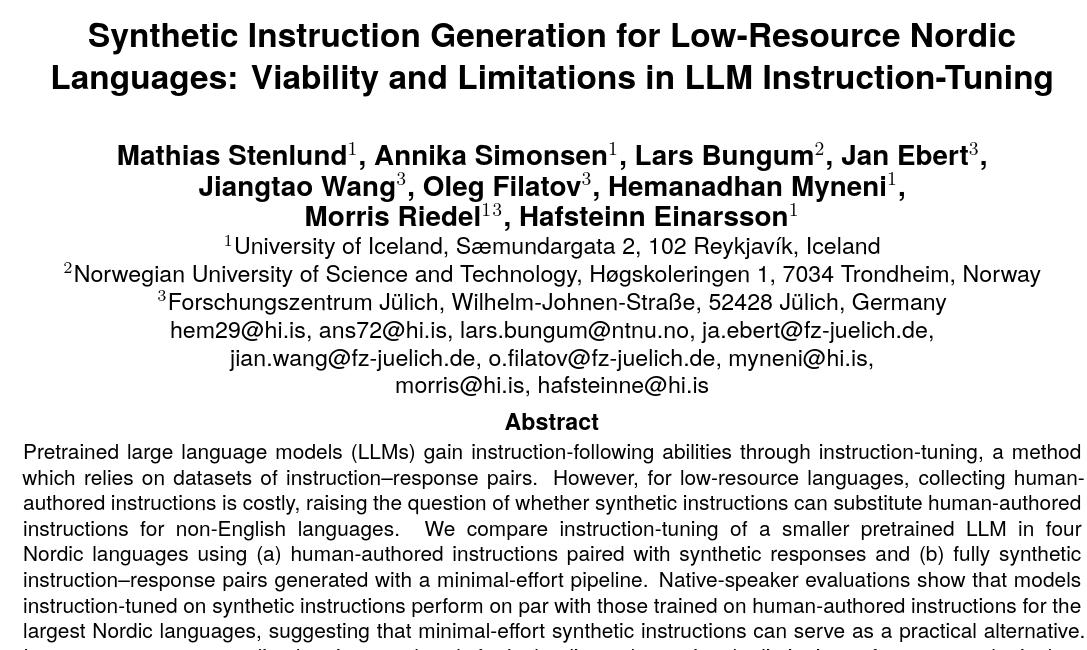
\includegraphics[height=1.15cm]{graphics/trustllm}\hspace*{3.5em}
        \includegraphics[height=1.15cm]{graphics/openwebsearch}\\[1.5ex]
        \color{DarkGreen}\scshape
        more coordination among eu initiatives\\[0.5ex]
%        e.g.\ openeurollm, openwebsearch, lds, etc.
      \end{center}
    \end{column}
  \end{columns}
\end{frame}

\begin{frame}[fragile]\includelogo
  \frametitle{Contact}
  \vspace*{4ex}
  \begin{columns}
    \begin{column}{0.5\textwidth}
      \begin{center}\color{DarkGreen}
        \textbf{Jan Haji\v{c}}\\[1.5ex]
        Charles University\\[1.5ex]
        \texttt{hajic@ufal.mff.cuni.cz}
      \end{center}
    \end{column}
    \begin{column}{0.5\textwidth}
      \begin{center}\color{DarkGreen}
        \textbf{Stephan Oepen}\\[1.5ex]
        University of Oslo\\[1.5ex]
        \texttt{oe@ifi.uio.no}
      \end{center}
    \end{column}
  \end{columns}
  \vspace*{5ex}
  \begin{center}
    \fboxsep 0pt
    \fbox{\includegraphics[height=7ex]{graphics/eu}}\\[1ex]
    \alert{\url{https://openeurollm.eu/}}
  \end{center}

\end{frame}

\end{document}

